%%%%%%%%%%%%%%%%%%%%%%%%%%%%%%%%%%%%%%%%%%%%%%%%%%%%%%%%%%%%%%%%%%%%%%%%%%%%%%%%%%%%%%%%%%%%%%%%%%%
%%%%%%%%%%%%%%%%%%%%%%%%%%%%%%%%%%%%%%%%%%%%%%%%%%%%%%%%%%%%%%%%%%%%%%%%%%%%%%%%%%%%%%%%%%%%%%%%%%%
%%%%%%%%%%%%%%%%%%%%%%%%%%%%%%%%%%%%%%%%%%%%%%%%%%%%%%%%%%%%%%%%%%%%%%%%%%%%%%%%%%%%%%%%%%%%%%%%%%%

\chapter{Cuadros y figuras adicionales}
\label{apendiceA}

En este apéndice se muestran mayores detalles sobre los resultados obtenidas durante los análisis descritos en el capítulo \ref{ch:metodologia}.
%
Este material fue excluido del texto principal con el fin de agilizar su lectura y enfatizar la interpretación de los resultados en el contexto del PDCL, más que la forma en que fueron calculados.

Los gráficos \ref{a:cabezas_ctrl} y \ref{a:cabezas_pdcl} representan, esquemáticamente, las derivaciones donde las proporciones de épocas estacionarias son diferentes en MOR y NMOR; para más detalles ver la sección \ref{sec:analisis_epoca}.
%
Estos gráficos pueden entenderse como una réplica de la figura \ref{cabeza_new} usando varios tamaños de época.

%Por fines de enfatizar las tendencias halladas, 
%
%En este apéndice se muestran los compilados gráficos mencionados en la parte de resultados,
%y que representan la
%distribución temporal y pseudo-espacial de las ocurrencia de épocas PSG dentro de los registros 
%para cada paciente. 

%Primeramente se presentan los compilados gráficos en los que se ha destacado el sueño MOR;
%posteriormente se presentan los mismos gráficos resaltando los patrones visuales
%propuestos, que parecen estar relacionados con la aparición de sueño MOR.

Como prueba voy a referirme a las figuras \cref{test1,test2,test3,test4,test5}.

%\begin{figure}
%\centering
%{\small
%\begin{tabular}{lccccc}
%\toprule
%{\small Tamaño de} & \multicolumn{5}{c}{Grupo CTRL} \\
%    \cmidrule{2-6}
%{\small ventana [s]}    & VCR & MJH & JAE & GHA & MFGR \\
%\midrule
%$30 \times 2^1$ &
%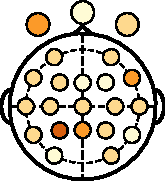
\includegraphics[width=0.13\textwidth]{./img_art_dfa/cabeza_new_VCR_60.pdf} &
%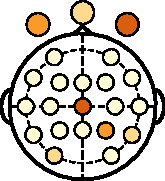
\includegraphics[width=0.13\textwidth]{./img_art_dfa/cabeza_new_MJH_60.pdf} &
%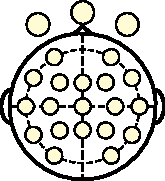
\includegraphics[width=0.13\textwidth]{./img_art_dfa/cabeza_new_JAE_60.pdf} &
%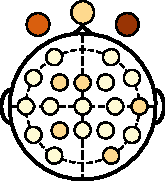
\includegraphics[width=0.13\textwidth]{./img_art_dfa/cabeza_new_GHA_60.pdf} &
%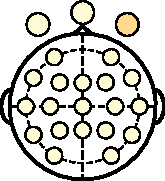
\includegraphics[width=0.13\textwidth]{./img_art_dfa/cabeza_new_MFGR_60.pdf} \\
%\midrule
%$30 \times 2^0$ &
%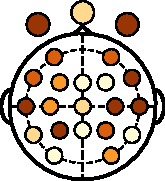
\includegraphics[width=0.13\textwidth]{./img_art_dfa/cabeza_new_VCR_30.pdf} &
%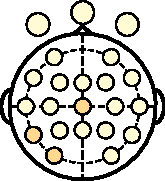
\includegraphics[width=0.13\textwidth]{./img_art_dfa/cabeza_new_MJH_30.pdf} &
%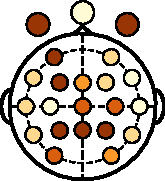
\includegraphics[width=0.13\textwidth]{./img_art_dfa/cabeza_new_JAE_30.pdf} &
%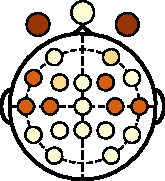
\includegraphics[width=0.13\textwidth]{./img_art_dfa/cabeza_new_GHA_30.pdf} &
%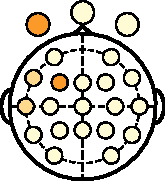
\includegraphics[width=0.13\textwidth]{./img_art_dfa/cabeza_new_MFGR_30.pdf} \\
%\midrule
%$30 \times 2^{-1}$ &
%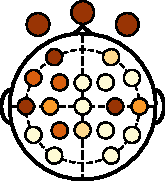
\includegraphics[width=0.13\textwidth]{./img_art_dfa/cabeza_new_VCR_15.pdf} &
%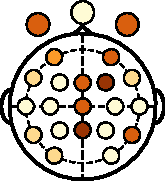
\includegraphics[width=0.13\textwidth]{./img_art_dfa/cabeza_new_MJH_15.pdf} &
%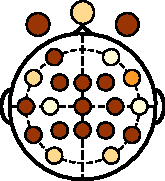
\includegraphics[width=0.13\textwidth]{./img_art_dfa/cabeza_new_JAE_15.pdf} &
%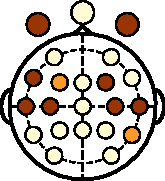
\includegraphics[width=0.13\textwidth]{./img_art_dfa/cabeza_new_GHA_15.pdf} &
%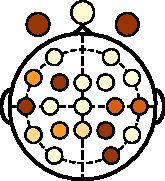
\includegraphics[width=0.13\textwidth]{./img_art_dfa/cabeza_new_MFGR_15.pdf} \\
%\bottomrule
%\end{tabular}\\
%
\includegraphics[scale=.7]{./img_art_dfa/escala.pdf} \\
%}
%\caption{Derivaciones para las cuales la proporción de épocas clasificadas como estacionarias fue significativamente diferente en MOR y NMOR.
%%
%Se han usado diferentes tamaños de ventana.
%%
%La posición de los círculos representan a las derivaciones, en correspondencia con la figura \ref{img:estampa}.}
%\label{a:cabezas_ctrl}
%\end{figure}

%\begin{figure}
%\centering
%{\small
%\begin{tabular}{lccccc}
%\toprule
%{ Tamaño de} & \multicolumn{5}{c}{Grupo PDCL} \\
%    \cmidrule{2-6}
%{ ventana [s]}    & CLO & RLO & RRU & JGZ & AEFP \\
%\midrule
%$30 \times 2^1$ &
%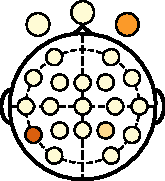
\includegraphics[width=0.13\textwidth]{./img_art_dfa/cabeza_new_CLO_60.pdf} &
%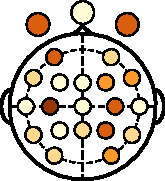
\includegraphics[width=0.13\textwidth]{./img_art_dfa/cabeza_new_RLO_60.pdf} &
%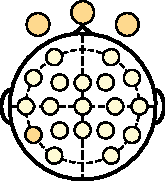
\includegraphics[width=0.13\textwidth]{./img_art_dfa/cabeza_new_RRU_60.pdf} &
%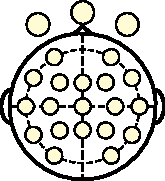
\includegraphics[width=0.13\textwidth]{./img_art_dfa/cabeza_new_JGZ_60.pdf} &
%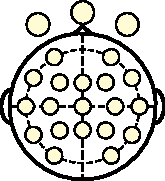
\includegraphics[width=0.13\textwidth]{./img_art_dfa/cabeza_new_AEFP_60.pdf} \\
%\midrule
%$30 \times 2^0$ &
%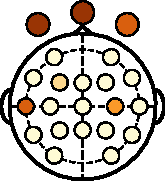
\includegraphics[width=0.13\textwidth]{./img_art_dfa/cabeza_new_CLO_30.pdf} &
%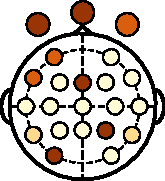
\includegraphics[width=0.13\textwidth]{./img_art_dfa/cabeza_new_RLO_30.pdf} &
%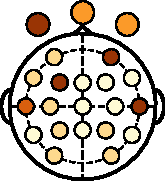
\includegraphics[width=0.13\textwidth]{./img_art_dfa/cabeza_new_RRU_30.pdf} &
%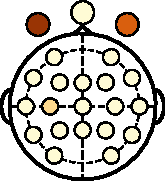
\includegraphics[width=0.13\textwidth]{./img_art_dfa/cabeza_new_JGZ_30.pdf} &
%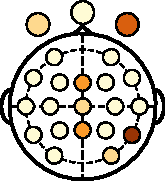
\includegraphics[width=0.13\textwidth]{./img_art_dfa/cabeza_new_AEFP_30.pdf} \\
%\midrule
%$30 \times 2^{-1}$ &
%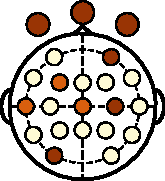
\includegraphics[width=0.13\textwidth]{./img_art_dfa/cabeza_new_CLO_15.pdf} &
%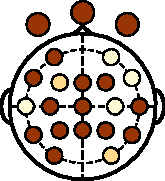
\includegraphics[width=0.13\textwidth]{./img_art_dfa/cabeza_new_RLO_15.pdf} &
%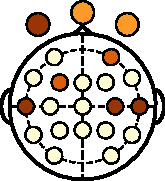
\includegraphics[width=0.13\textwidth]{./img_art_dfa/cabeza_new_RRU_15.pdf} &
%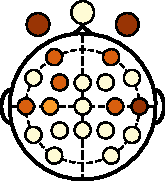
\includegraphics[width=0.13\textwidth]{./img_art_dfa/cabeza_new_JGZ_15.pdf} &
%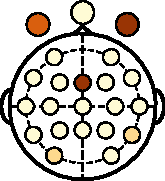
\includegraphics[width=0.13\textwidth]{./img_art_dfa/cabeza_new_AEFP_15.pdf} \\
%\bottomrule
%\end{tabular} \\
%
\includegraphics[scale=.7]{./img_art_dfa/escala.pdf} \\
%}
%\caption{Derivaciones para las cuales la proporción de épocas clasificadas como estacionarias fue significativamente diferente en MOR y NMOR.
%%
%Se han usado diferentes tamaños de ventana.
%%
%La posición de los círculos representan a las derivaciones, en correspondencia con la figura \ref{img:estampa}.}
%\label{a:cabezas_pdcl}
%\end{figure}

%%%%%%%%%%%%%%%%%%%%%%%%%%%%%%%%%%%%%%%%%%%%%%%%%%%%%%%%%%%%%%%%%%%%%%%%%%%%%%%%%%%%%%%%%%%%%%%%%%%
%%%%%%%%%%%%%%%%%%%%%%%%%%%%%%%%%%%%%%%%%%%%%%%%%%%%%%%%%%%%%%%%%%%%%%%%%%%%%%%%%%%%%%%%%%%%%%%%%%%

\begin{SidewaysTable}
\centering
\caption{Épocas estacionarias, participante VCR}
{\small
\begin{tabular}{lrrrlrrrlrrrlrrrlrrrlrrr}
\toprule
      & \multicolumn{3}{l}{E = 0.9375} &  & \multicolumn{3}{l}{E = 1.875} &  & \multicolumn{3}{l}{E = 3.75} &  & \multicolumn{3}{l}{E = 7.5} &  & \multicolumn{3}{l}{E = 15} &  & \multicolumn{3}{l}{E = 30} \\
\cmidrule{2-4} \cmidrule{6-8} \cmidrule{10-12} \cmidrule{14-16} \cmidrule{18-20}
      & N+W       & R       & P        &  & N+W      & R       & P        &  & N+W      & R      & P        &  & N+W     & R      & P        &  & N+W     & R      & P       &  & N+W     & R     & P        \\
\midrule
Fp2   & 11789     & 1258    & .000    &  & 5801     & 604     & .001    &  & 3200     & 263    & .018    &  & 1455    & 80     & .000    &  & 545     & 22     & .000   &  & 188     & 3     & .000    \\
Fp1   & 11112     & 1232    & .000    &  & 5674     & 620     & .000    &  & 3058     & 256    & .054    &  & 1463    & 82     & .000    &  & 549     & 15     & .000   &  & 204     & 2     & .000    \\
F8    & 12067     & 1378    & .000    &  & 6669     & 651     & .088    &  & 3643     & 324    & .353    &  & 1581    & 132    & .156    &  & 615     & 39     & .009   &  & 223     & 4     & .000    \\
F7    & 12513     & 1323    & .000    &  & 6892     & 670     & .104    &  & 3648     & 293    & .001    &  & 1537    & 99     & .000    &  & 595     & 34     & .002   &  & 216     & 8     & .007    \\
F4    & 9748      & 1033    & .000    &  & 5779     & 565     & .129    &  & 3505     & 329    & .772    &  & 1583    & 146    & 1.000    &  & 605     & 46     & .157   &  & 246     & 18    & .347    \\
F3    & 11457     & 1365    & .000    &  & 6384     & 727     & .000    &  & 3535     & 354    & .055    &  & 1584    & 143    & .753    &  & 620     & 38     & .005   &  & 225     & 7     & .002    \\
T4    & 12480     & 1461    & .000    &  & 7426     & 796     & .000    &  & 4006     & 418    & .000    &  & 1745    & 188    & .007    &  & 649     & 65     & .524   &  & 245     & 15    & .109    \\
T3    & 13432     & 1479    & .000    &  & 7673     & 845     & .000    &  & 3752     & 425    & .000    &  & 1694    & 186    & .003    &  & 650     & 65     & .533   &  & 237     & 14    & .093    \\
C4    & 11326     & 1243    & .000    &  & 6726     & 710     & .000    &  & 3706     & 353    & .489    &  & 1624    & 124    & .008    &  & 599     & 32     & .001   &  & 208     & 6     & .002    \\
C3    & 11947     & 1355    & .000    &  & 7059     & 759     & .000    &  & 3860     & 396    & .004    &  & 1681    & 163    & .484    &  & 637     & 45     & .046   &  & 238     & 8     & .002    \\
T6    & 12975     & 1450    & .000    &  & 7823     & 836     & .000    &  & 4027     & 431    & .000    &  & 1857    & 157    & .135    &  & 752     & 52     & .013   &  & 271     & 20    & .325    \\
T5    & 13267     & 1450    & .000    &  & 7668     & 852     & .000    &  & 3730     & 419    & .000    &  & 1993    & 200    & .111    &  & 796     & 69     & .551   &  & 303     & 17    & .025    \\
P4    & 11948     & 1399    & .000    &  & 7311     & 818     & .000    &  & 4032     & 409    & .007    &  & 1707    & 155    & .801    &  & 655     & 41     & .005   &  & 218     & 5     & .000    \\
P3    & 12035     & 1363    & .000    &  & 7273     & 845     & .000    &  & 3880     & 410    & .000    &  & 1661    & 166    & .231    &  & 616     & 57     & 1.000   &  & 224     & 8     & .004    \\
O2    & 10415     & 1254    & .000    &  & 6716     & 769     & .000    &  & 3816     & 406    & .000    &  & 1954    & 209    & .003    &  & 695     & 66     & .876   &  & 272     & 14    & .019    \\
O1    & 11418     & 1377    & .000    &  & 6753     & 812     & .000    &  & 3648     & 415    & .000    &  & 1901    & 218    & .000    &  & 758     & 79     & .231   &  & 288     & 22    & .380    \\
FZ    & 10204     & 1280    & .000    &  & 5924     & 635     & .000    &  & 3398     & 356    & .003    &  & 1585    & 136    & .297    &  & 606     & 37     & .005   &  & 224     & 9     & .009    \\
CZ    & 10772     & 1189    & .000    &  & 6333     & 628     & .034    &  & 3671     & 342    & .906    &  & 1628    & 128    & .023    &  & 609     & 43     & .054   &  & 221     & 5     & .000    \\
PZ    & 11300     & 1241    & .000    &  & 6800     & 770     & .000    &  & 3780     & 418    & .000    &  & 1666    & 163    & .400    &  & 592     & 45     & .164   &  & 207     & 7     & .005    \\
LOG   & 8922      & 1043    & .000    &  & 5462     & 545     & .044    &  & 3265     & 246    & .000    &  & 1820    & 107    & .000    &  & 832     & 35     & .000   &  & 320     & 11    & .000    \\
ROG   & 8688      & 882     & .003    &  & 5183     & 465     & .458    &  & 3118     & 231    & .000    &  & 1739    & 96     & .000    &  & 779     & 31     & .000   &  & 310     & 11    & .000    \\
EMG   & 20131     & 1636    & .000    &  & 8808     & 772     & .017    &  & 3769     & 350    & .969    &  & 1442    & 174    & .000    &  & 414     & 65     & .000   &  & 122     & 20    & .028    \\
Total & 25236     & 2336    &          &  & 12618    & 1168    &          &  & 6309     & 584    &          &  & 3154    & 292    &          &  & 1577    & 146    &         &  & 788     & 73    &          \\ \bottomrule
\end{tabular}
}
\end{SidewaysTable}

%%%%%%%%%%%%%%%%%%%%%%%%%%%%%%%%%%%%%%%%%%%%%%%%%%%%%%%%%%%%%%%%%%%%%%%%%%%%%%%%%%%%%%%%%%%%%%%%%%%
%%%%%%%%%%%%%%%%%%%%%%%%%%%%%%%%%%%%%%%%%%%%%%%%%%%%%%%%%%%%%%%%%%%%%%%%%%%%%%%%%%%%%%%%%%%%%%%%%%%

\begin{figure}
\begin{subfigure}{\textwidth}
\centering
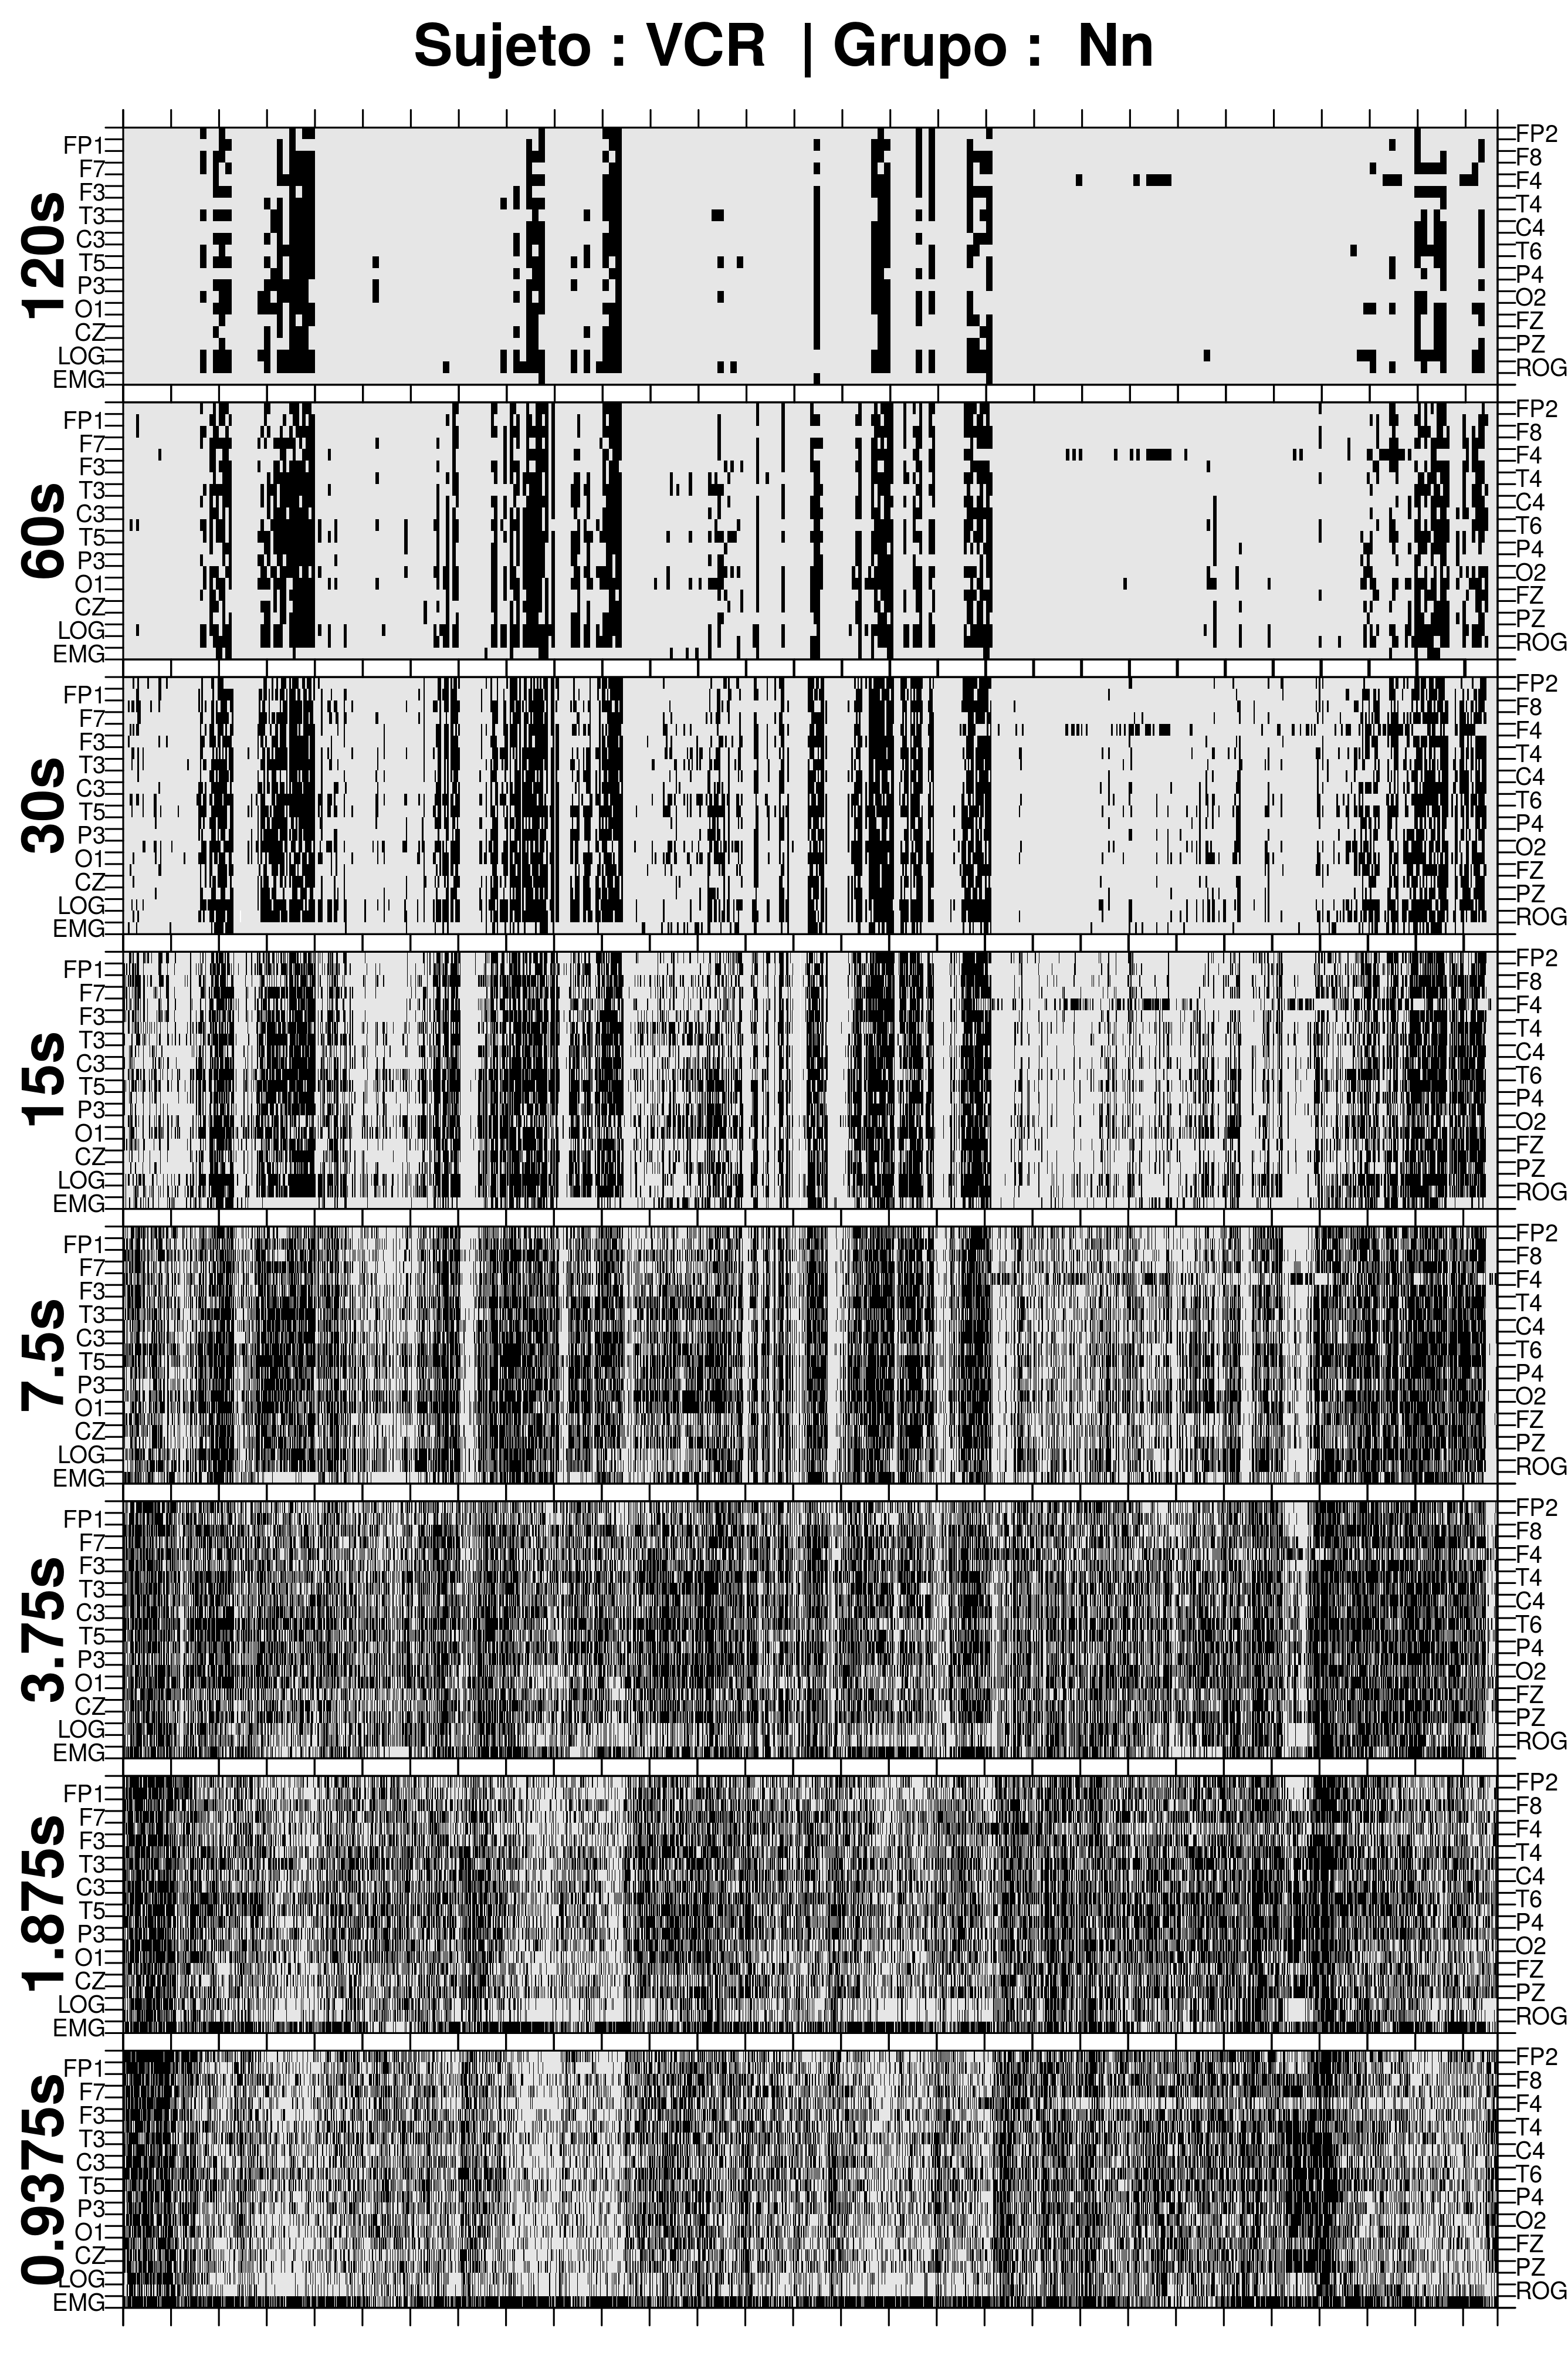
\includegraphics[width=.9\linewidth]
{./img_ejemplos/VCNNS1_comp_est_.png} 
\caption{Épocas estacionarias usando diferentes tamaños de ventana}
\end{subfigure}
\end{figure}

%\begin{figure}
%\ContinuedFloat
%\begin{subfigure}{\linewidth}
%\centering
%\includegraphics[width=0.9\linewidth]
%{./enlentecimiento/VCNNS1_espectral_total.png} 
%\caption{Espectro de potencias de banda ancha}
%\end{subfigure}
%\end{figure}

%\begin{figure}
%\ContinuedFloat
%\begin{subfigure}{\linewidth}
%\centering
%\includegraphics[width=0.9\linewidth]
%{./img_resultados/VCNNS1_combinado_.png} 
%\caption{Espectro de potencias y análisis de estacionariedad para los canales LOG, ROG y EMG}
%\end{subfigure}
%\end{figure}

\begin{figure}
\ContinuedFloat
\begin{subfigure}{\linewidth}
\centering
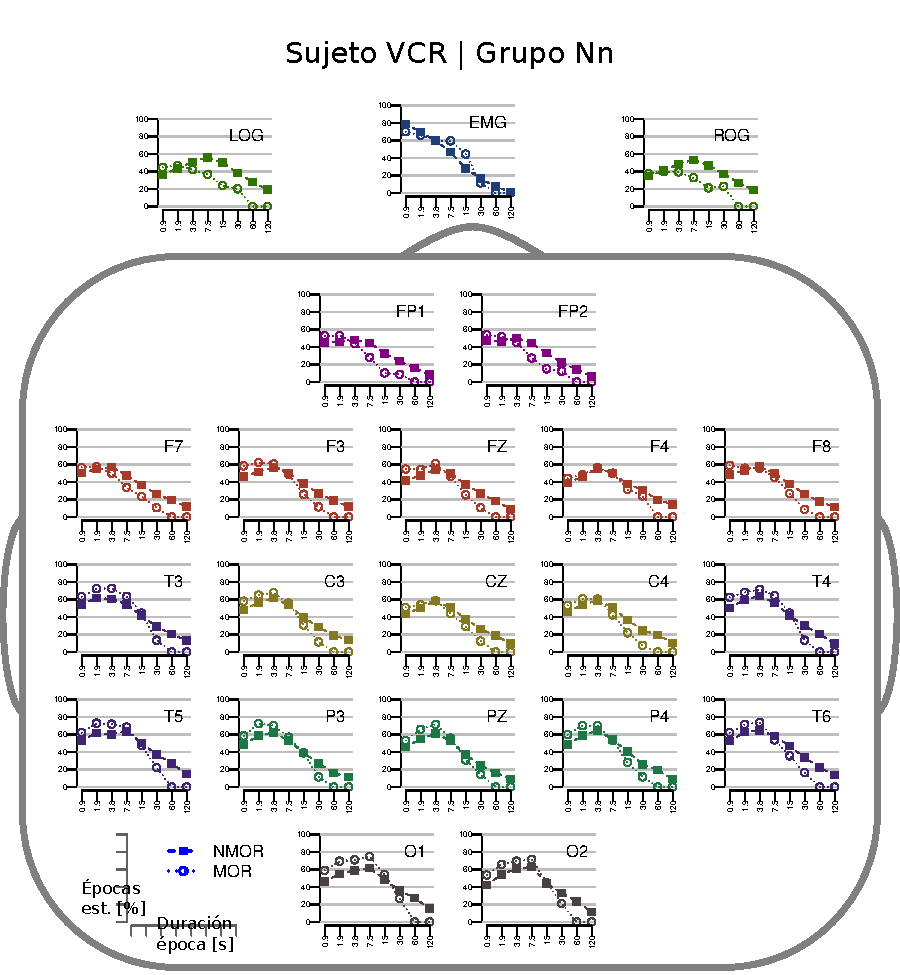
\includegraphics[width=.9\linewidth]{./img_resultados/cabeza_VCR.pdf}
%\caption{Porcentajes de épocas estacionarias, VCR (VCNNS1)}
\caption{Resumen de épocas estacionarias según tamaño de ventana}
\end{subfigure}
\caption{Gráficos individuales para el sujeto VCR}
\end{figure}

%%%%%%%%%%%%%%%%%%%%%%%%%%%%%%%%%%%%%%%%%%%%%%%%%

%\begin{figure}
%\centering
%\includegraphics[width=0.9\linewidth]
%{./img_ejemplos/MJNNVIGILOS_comp_est_.png} 
%\end{figure}
%
%\begin{figure}
%\centering
%\includegraphics[width=0.9\linewidth]
%{./enlentecimiento/MJNNVIGILOS_espectral_total.png} 
%\end{figure}
%
%\begin{figure}
%\centering
%\includegraphics[width=0.9\linewidth]
%{./img_resultados/MJNNVIGILOS_combinado_.png} 
%\end{figure}
%
%\begin{figure}
%\centering
%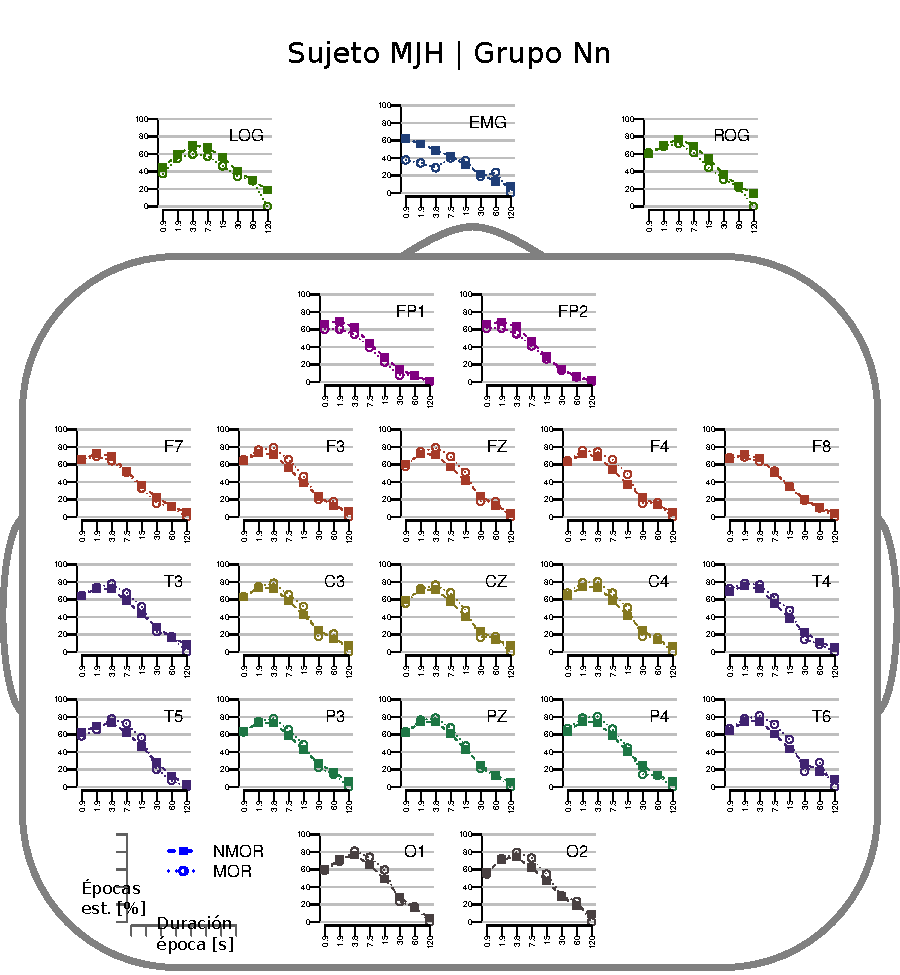
\includegraphics[width=.9\linewidth]{./img_resultados/cabeza_MJH.pdf}
%%\caption{Porcentajes de épocas estacionarias, MJH (MJNNVIGILOS)}
%\end{figure}
%
%%%%%%%%%%%%%%%%%%%%%%%%%%%%%%%%%%%%%%%%%%%%%%%%%%
%
%\begin{figure}
%\centering
%\includegraphics[width=0.9\linewidth]
%{./img_ejemplos/JANASUE_comp_est_.png} 
%\end{figure}
%\begin{figure}
%\centering
%\includegraphics[width=0.9\linewidth]
%{./enlentecimiento/JANASUE_espectral_total.png} 
%\end{figure}
%\begin{figure}
%\centering
%\includegraphics[width=0.9\linewidth]
%{./img_resultados/JANASUE_combinado_.png} 
%\end{figure}
%
%\begin{figure}
%\centering
%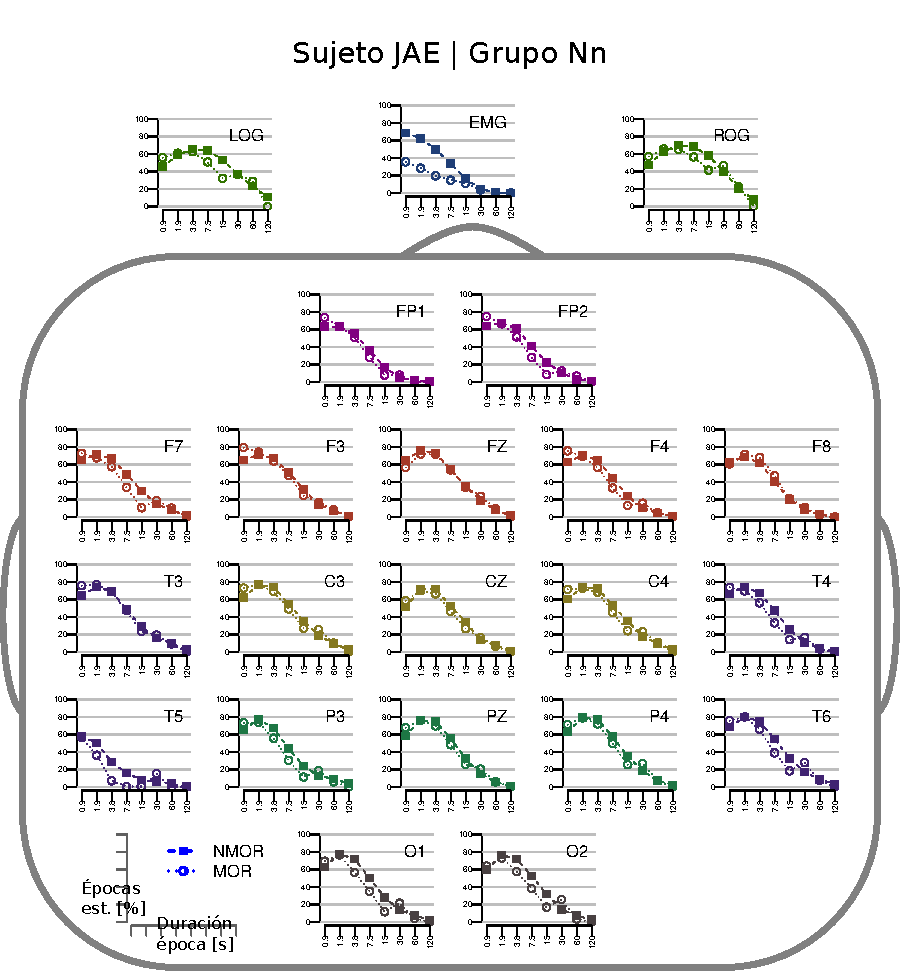
\includegraphics[width=.9\linewidth]{./img_resultados/cabeza_JAE.pdf}
%%\caption{Porcentajes de épocas estacionarias, JAE (JANASUE)}
%\end{figure}
%
%%%%%%%%%%%%%%%%%%%%%%%%%%%%%%%%%%%%%%%%%%%%%%%%%%
%
%\begin{figure}
%\centering
%\includegraphics[width=0.9\linewidth]
%{./img_ejemplos/GH24031950SUENO_comp_est_.png} 
%\end{figure}
%\begin{figure}
%\centering
%\includegraphics[width=0.9\linewidth]
%{./enlentecimiento/GH24031950SUENO_espectral_total.png} 
%\end{figure}
%\begin{figure}
%\centering
%\includegraphics[width=0.9\linewidth]
%{./img_resultados/GH24031950SUENO_combinado_.png} 
%\end{figure}
%
%\begin{figure}
%\centering
%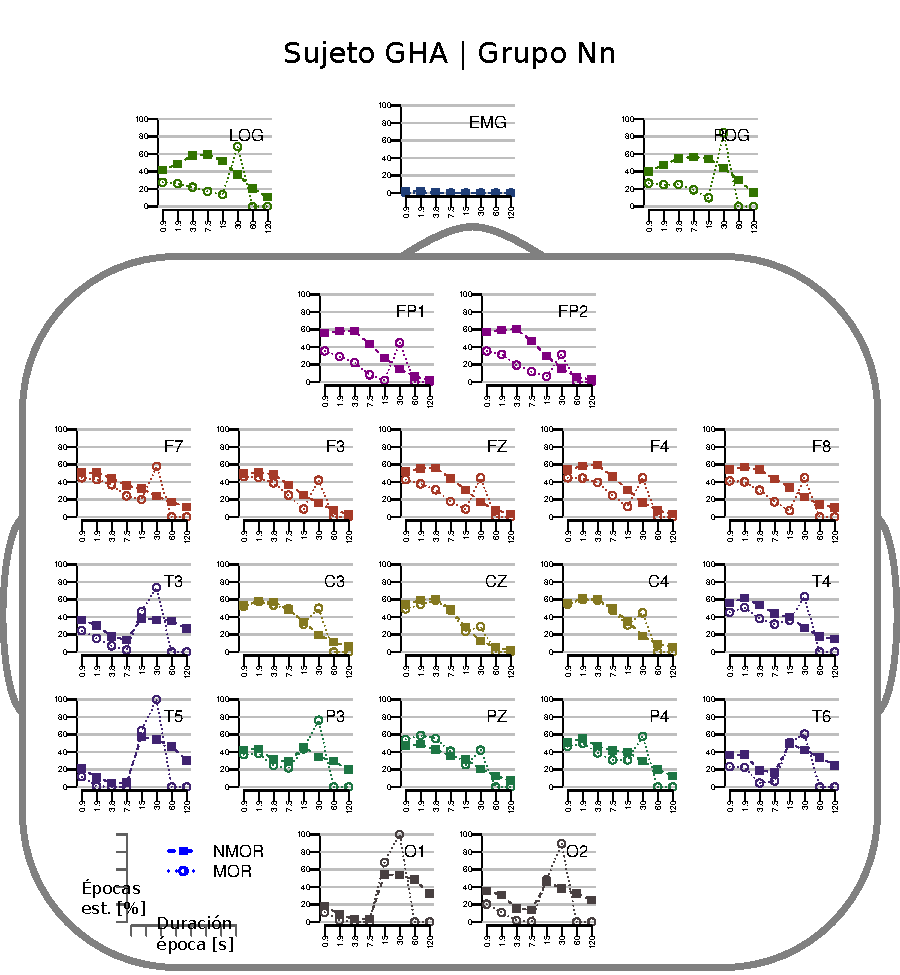
\includegraphics[width=.9\linewidth]{./img_resultados/cabeza_GHA.pdf}
%%\caption{Porcentajes de épocas estacionarias, GHA (GH24031950SUEÑO)}
%\end{figure}
%
%%%%%%%%%%%%%%%%%%%%%%%%%%%%%%%%%%%%%%%%%%%%%%%%%%
%
%\begin{figure}
%\centering
%\includegraphics[width=0.9\linewidth]
%{./img_ejemplos/GURM251148SUE_comp_est_.png} 
%\end{figure}
%\begin{figure}
%\centering
%\includegraphics[width=0.9\linewidth]
%{./enlentecimiento/GURM251148SUE_espectral_total.png} 
%\end{figure}
%\begin{figure}
%\centering
%\includegraphics[width=0.9\linewidth]
%{./img_resultados/GURM251148SUE_combinado_.png} 
%\end{figure}
%
%\begin{figure}
%\centering
%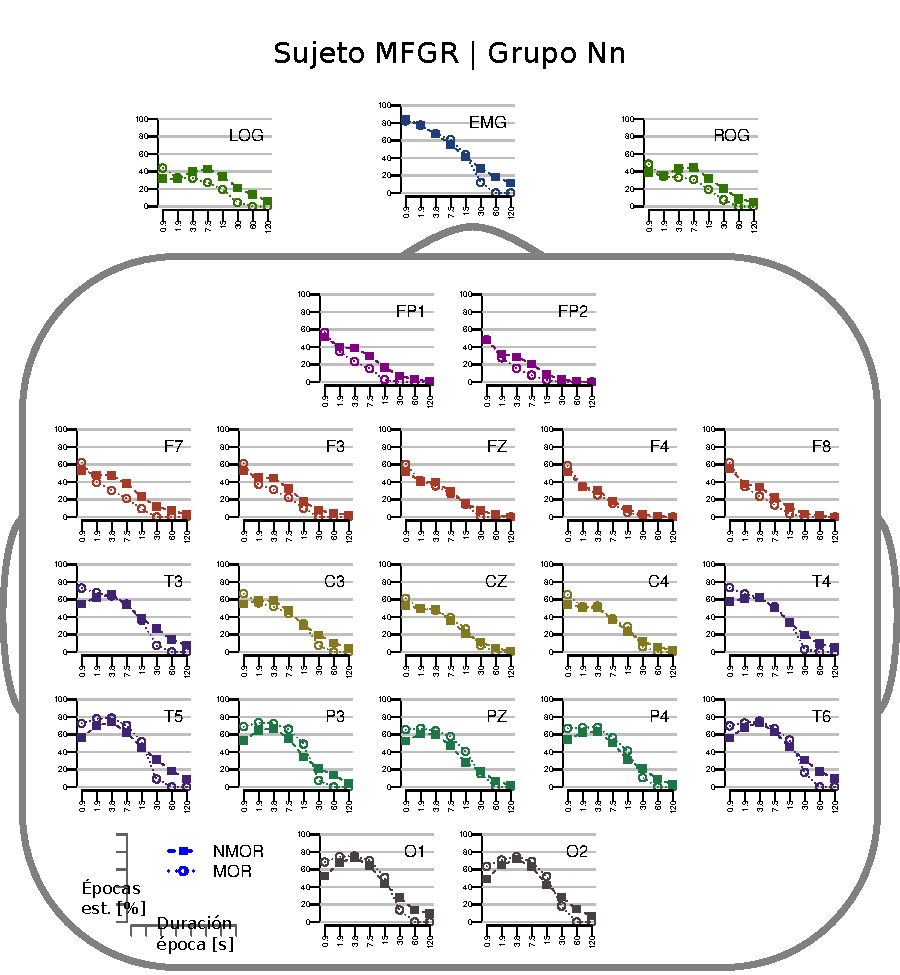
\includegraphics[width=.9\linewidth]{./img_resultados/cabeza_MFGR.pdf}
%%\caption{Porcentajes de épocas estacionarias MFGR (GURM251148SUE)}
%\end{figure}
%
%%%%%%%%%%%%%%%%%%%%%%%%%%%%%%%%%%%%%%
%%%%%%%%%%%%%%%%%%%%%%%%%%%%%%%%%%%%%%
%%%%%%%%%%%%%%%%%%%%%%%%%%%%%%%%%%%%%%
%
%\begin{figure}
%\centering
%\includegraphics[width=0.9\linewidth]
%{./img_ejemplos/CLMN10SUE_comp_est_.png} 
%\end{figure}
%
%\begin{figure}
%\centering
%\includegraphics[width=0.9\linewidth]
%{./enlentecimiento/CLMN10SUE_espectral_total.png} 
%\end{figure}
%
%\begin{figure}
%\centering
%\includegraphics[width=0.9\linewidth]
%{./img_resultados/CLMN10SUE_combinado_.png} 
%\end{figure}
%
%\begin{figure}
%\centering
%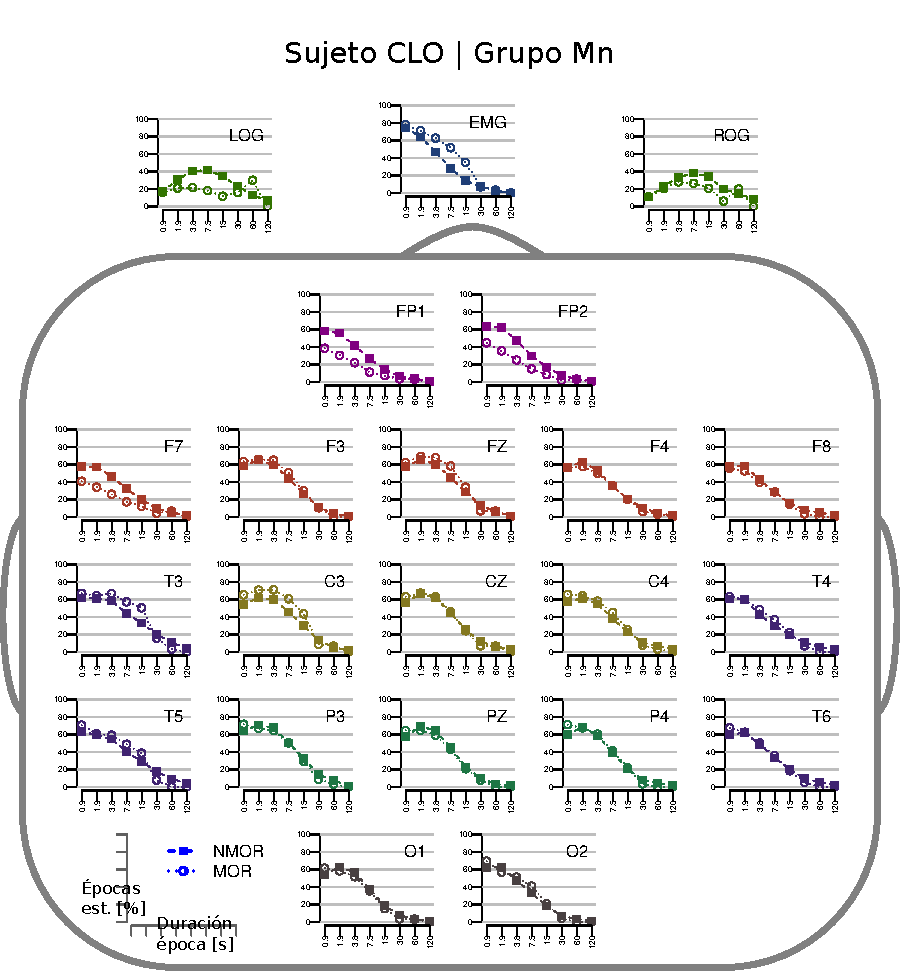
\includegraphics[width=.9\linewidth]{./img_resultados/cabeza_CLO.pdf}
%%\caption{Porcentajes de épocas estacionarias, CLO (CLMN10SUE)}
%\end{figure}
%
%%%%%%%%%%%%%%%%%%%%%%%%%%%%%%%%%%%%%%
%
%\begin{figure}
%\centering
%\includegraphics[width=0.9\linewidth]
%{./img_ejemplos/RLMN10SUE_comp_est_.png} 
%\end{figure}
%\begin{figure}
%\centering
%\includegraphics[width=0.9\linewidth]
%{./enlentecimiento/RLMN10SUE_espectral_total.png}
%\end{figure}
%\begin{figure}
%\centering
%\includegraphics[width=0.9\linewidth]
%{./img_ejemplos/RLMN10SUE_comp_est_.png} 
%\end{figure}
%
%\begin{figure}
%\centering
%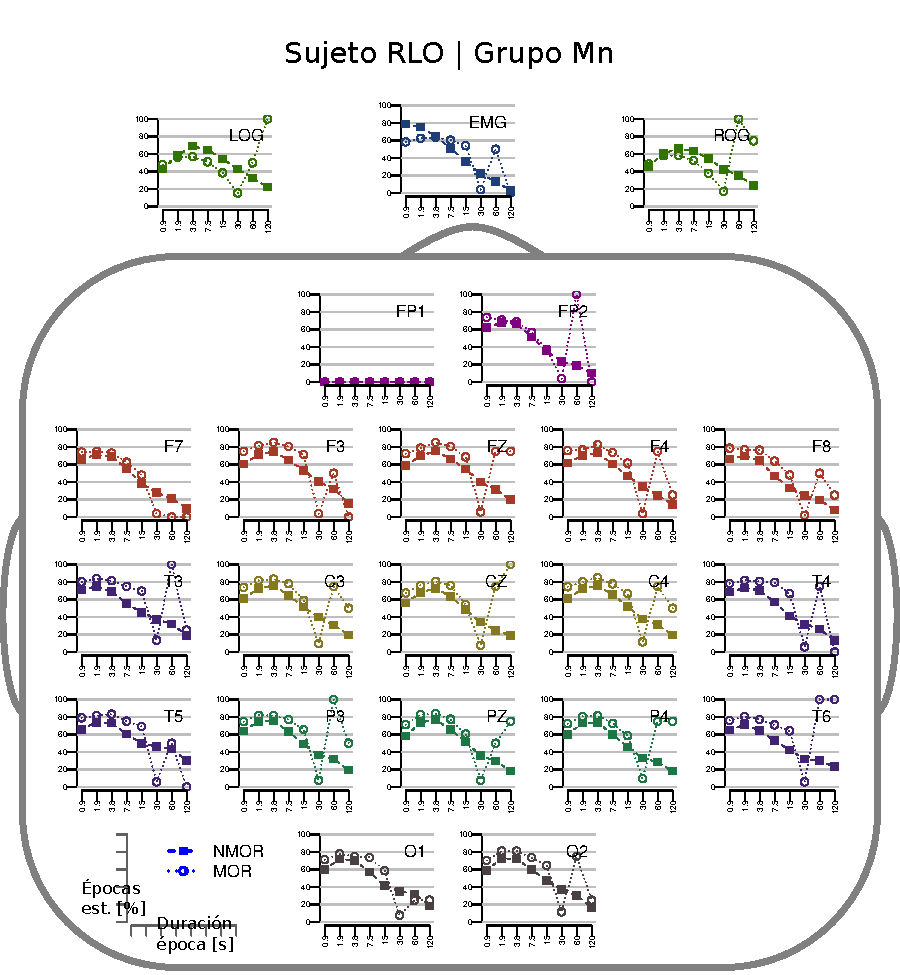
\includegraphics[width=.9\linewidth]{./img_resultados/cabeza_RLO.pdf}
%%\caption{Porcentajes de épocas estacionarias, RLO (RLMN10SUE)}
%\end{figure}
%
%%%%%%%%%%%%%%%%%%%%%%%%%%%%%%%%%%%%%%
%
%\begin{figure}
%\centering
%\includegraphics[width=0.9\linewidth]
%{./img_ejemplos/RRMNS_comp_est_.png} 
%\end{figure}
%
%\begin{figure}
%\centering
%\includegraphics[width=0.9\linewidth]
%{./enlentecimiento/RRMNS_espectral_total.png}
%\end{figure}
%
%\begin{figure}
%\centering
%\includegraphics[width=0.9\linewidth]
%{./img_resultados/RRMNS_combinado_.png} 
%\end{figure}
%
%\begin{figure}
%\centering
%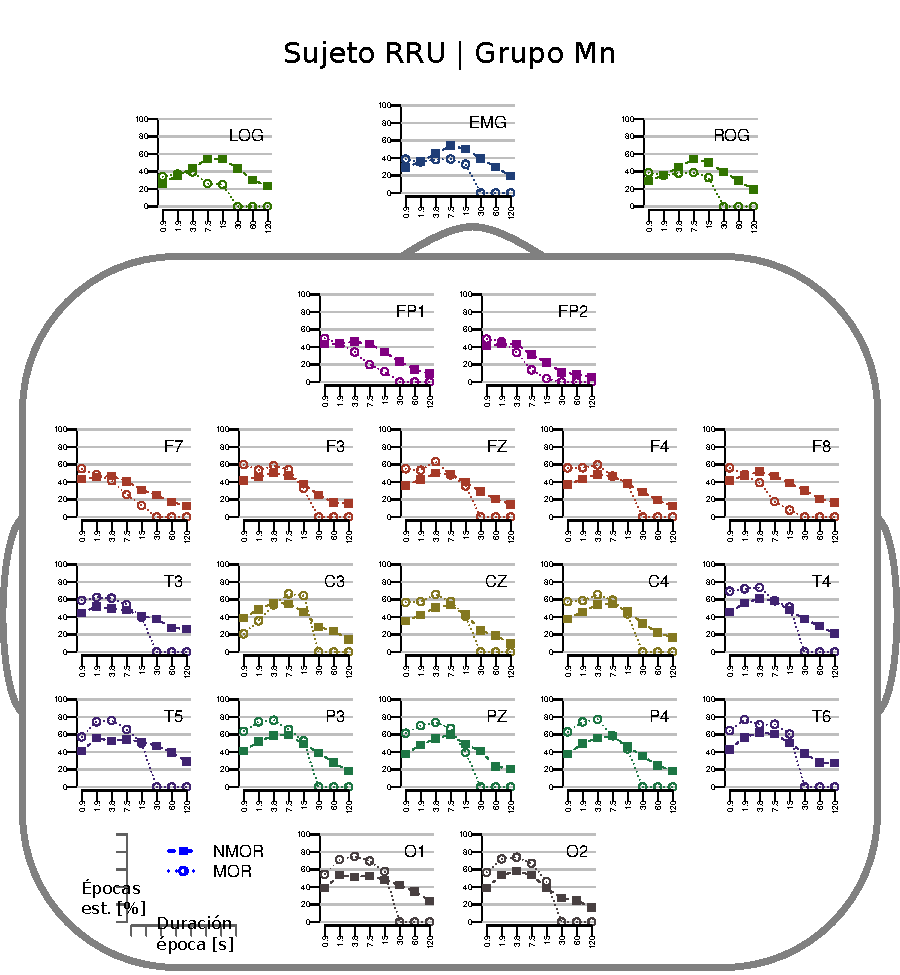
\includegraphics[width=.9\linewidth]{./img_resultados/cabeza_RRU.pdf}
%%\caption{Porcentajes de épocas estacionarias, RRU (RRMNS)}
%\end{figure}
%
%%%%%%%%%%%%%%%%%%%%%%%%%%%%%%%%%%%%%%
%
%\begin{figure}
%\centering
%\includegraphics[width=0.9\linewidth]
%{./img_ejemplos/JGMN6SUE_comp_est_.png} 
%\end{figure}
%
%\begin{figure}
%\centering
%\includegraphics[width=0.9\linewidth]
%{./enlentecimiento/JGMN6SUE_espectral_total.png} 
%\end{figure}
%
%\begin{figure}
%\centering
%\includegraphics[width=0.9\linewidth]
%{./img_resultados/JGMN6SUE_combinado_.png} 
%\end{figure}
%
%\begin{figure}
%\centering
%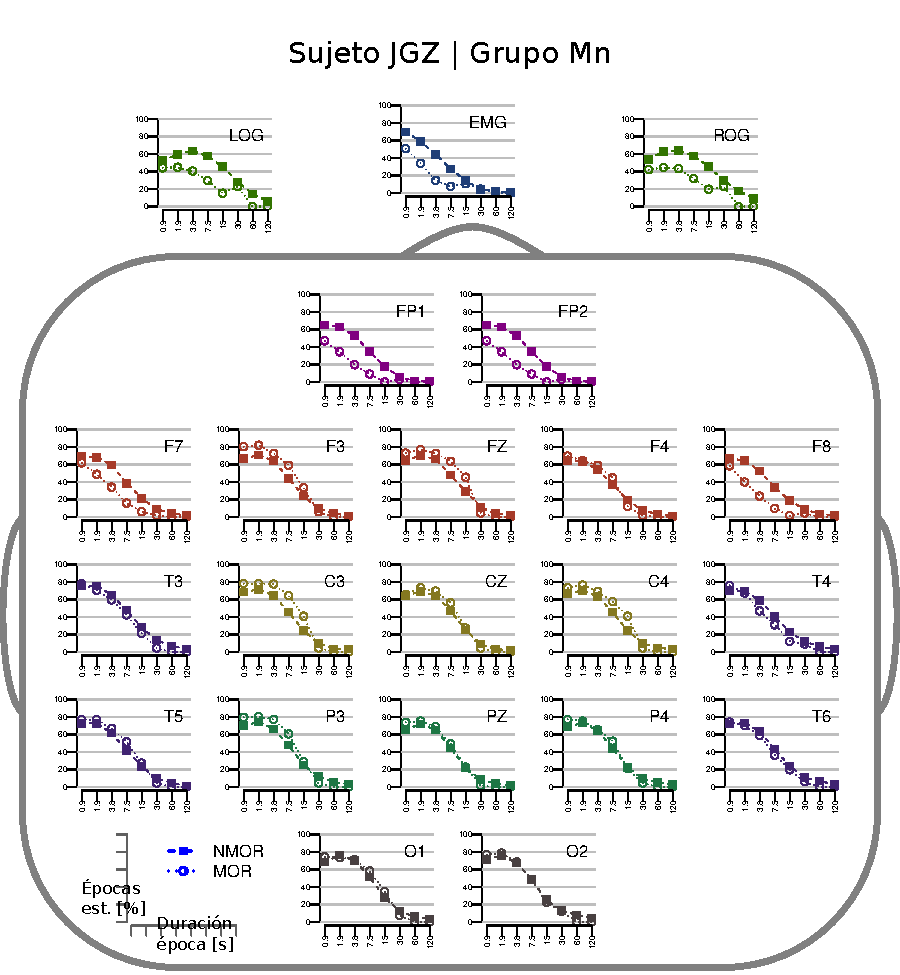
\includegraphics[width=.9\linewidth]{./img_resultados/cabeza_JGZ.pdf}
%%\caption{Porcentajes de épocas estacionarias, JGZ (JGMN6SUE)}
%\end{figure}
%
%%%%%%%%%%%%%%%%%%%%%%%%%%%%%%%%%%%%%%
%%%%%%%%%%%%%%%%%%%%%%%%%%%%%%%%%%%%%%
%%%%%%%%%%%%%%%%%%%%%%%%%%%%%%%%%%%%%%
%
%%\begin{figure}
%%\centering
%%\includegraphics[width=0.9\linewidth]
%%{./img_ejemplos/FGHSUE_comp_est_.png} 
%%\end{figure}
%%\begin{figure}
%%\centering
%%\includegraphics[width=0.9\linewidth]
%%{./img_resultados/FGHSUE_espectral_total.png} 
%%\end{figure}
%%\begin{figure}
%%\centering
%%\includegraphics[width=0.9\linewidth]
%%{./img_resultados/FGHSUE_combinado_.png} 
%%\end{figure}
%%
%%\begin{figure}
%%\centering
%%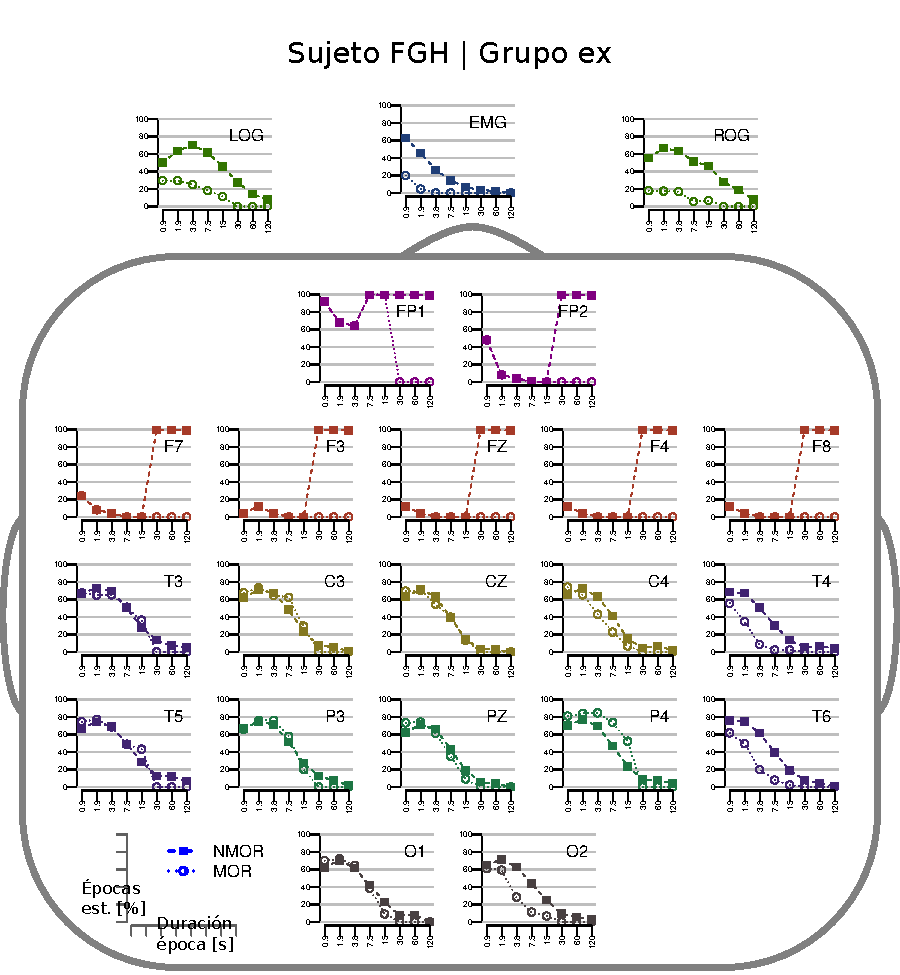
\includegraphics[width=.9\linewidth]{./img_resultados/cabeza_FGH.pdf}
%%%\caption{Porcentajes de épocas estacionarias, FGH (FGHSUE)}
%%\end{figure}
%
%%%%%%%%%%%%%%%%%%%%%%%%%%%%%%%%%%%%%%
%
%%\begin{figure}
%%\centering
%%\includegraphics[width=0.9\linewidth]
%%{./img_ejemplos/MGNA5SUE_comp_est_.png} 
%%\end{figure}
%%\begin{figure}
%%\centering
%%\includegraphics[width=0.9\linewidth]
%%{./img_resultados/MGNA5SUE_espectral_total.png} 
%%\end{figure}
%%\begin{figure}
%%\centering
%%\includegraphics[width=0.9\linewidth]
%%{./img_resultados/MGNA5SUE_combinado_.png} 
%%\end{figure}
%%
%%\begin{figure}
%%\centering
%%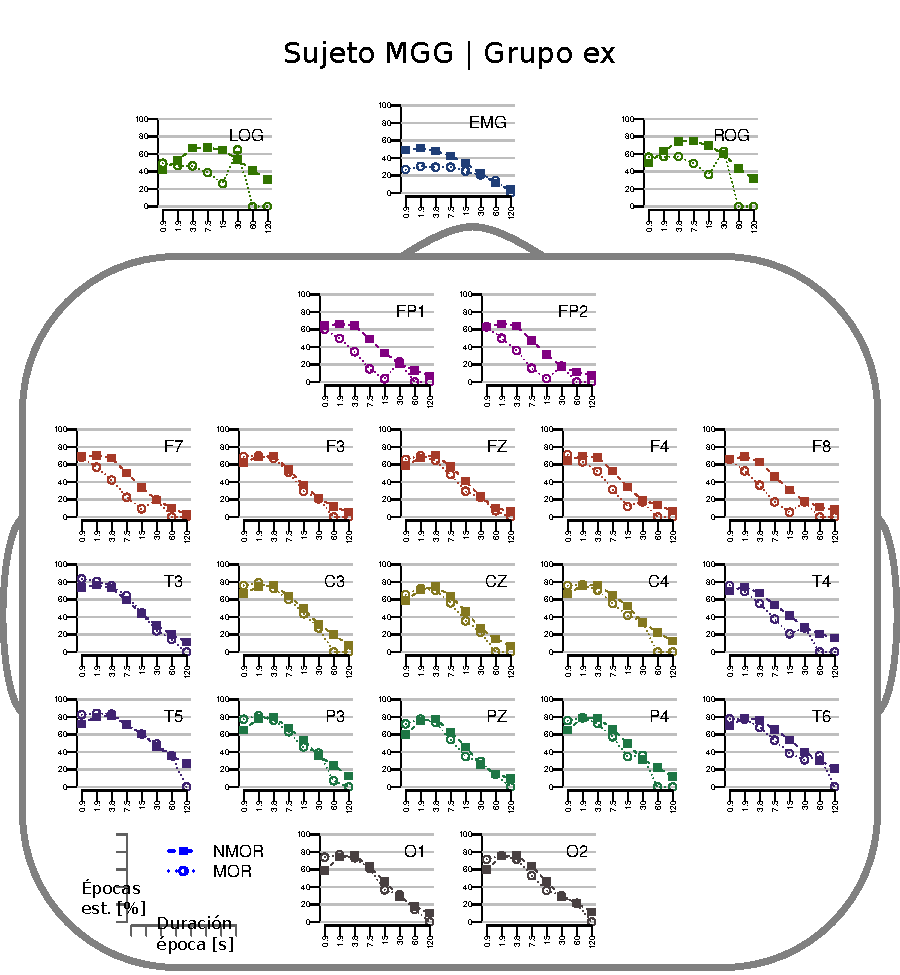
\includegraphics[width=.9\linewidth]{./img_resultados/cabeza_MGG.pdf}
%%%\caption{Porcentajes de épocas estacionarias, MGG (MGNA5SUE)}
%%\end{figure}
%
%%%%%%%%%%%%%%%%%%%%%%%%%%%%%%%%%%%%%%
%
%%\begin{figure}
%%\centering
%%\includegraphics[width=0.9\linewidth]
%%{./img_ejemplos/EMNNS_comp_est_.png} 
%%\end{figure}
%%\begin{figure}
%%\centering
%%\includegraphics[width=0.9\linewidth]
%%{./img_ejemplos/EMNNS_comp_est_.png} 
%%\end{figure}
%%\begin{figure}
%%\centering
%%\includegraphics[width=0.9\linewidth]
%%{./img_ejemplos/EMNNS_comp_est_.png} 
%%\end{figure}
%%
%%\begin{figure}
%%\centering
%%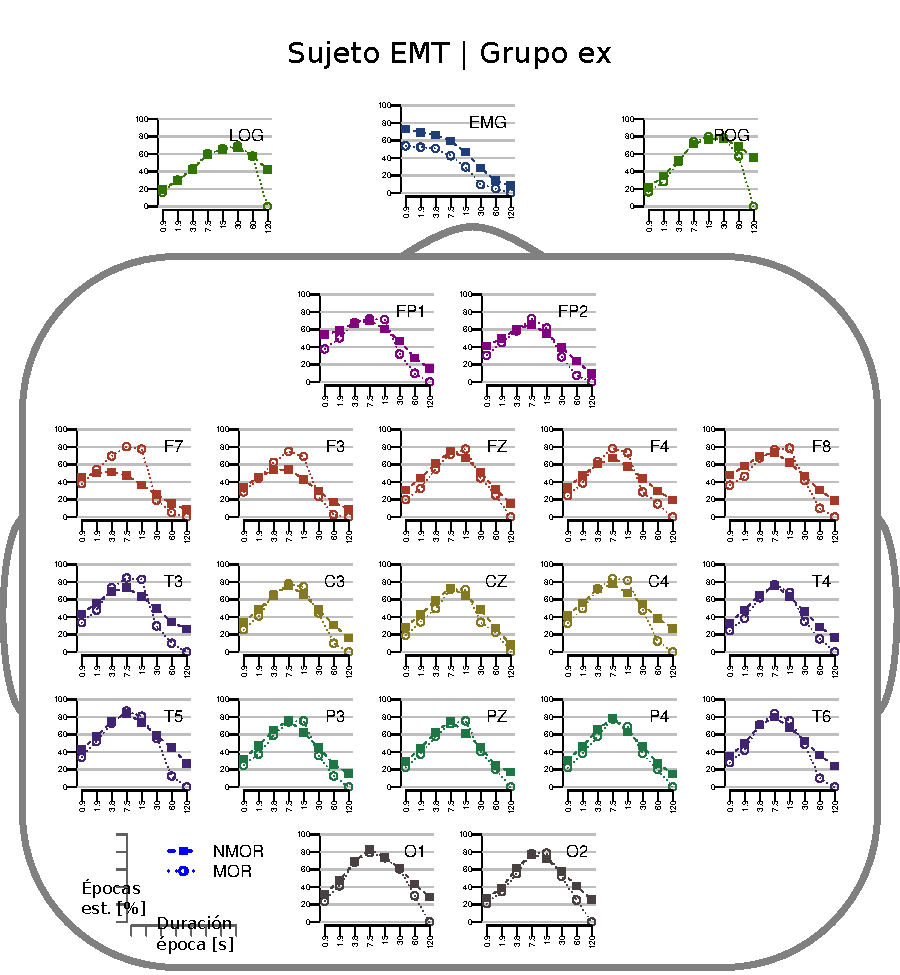
\includegraphics[width=.9\linewidth]{./img_resultados/cabeza_EMT.pdf}
%%%\caption{Porcentajes de épocas estacionarias EMT (EMNNS)}
%%\end{figure}
%
%%%%%%%%%%%%%%%%%%%%%%%%%%%%%%%%%%%%%%
%
%%\begin{figure}
%%\bordes{1.5}
%%\begin{tabular}{l}
%%\Large{{Patrones visuales}}\\
%%\begin{tabular}{c}
%%\includegraphics[width=0.45\textwidth]
%%{./img_ejemplos/zoom_VCR.pdf}
%%\includegraphics[width=0.45\textwidth]
%%{./img_ejemplos/zoom_MJH.pdf}
%%\\
%%\includegraphics[width=0.45\textwidth]
%%{./img_ejemplos/zoom_JAE.pdf}
%%\includegraphics[width=0.45\textwidth]
%%{./img_ejemplos/zoom_GHA.pdf}
%%\\
%%\includegraphics[width=0.45\textwidth]
%%{./img_ejemplos/zoom_MFGR.pdf}
%%\end{tabular}
%%\end{tabular}
%%\end{figure}
%

\begin{figure}
\Large{\textbf{Patrones visuales}}\\
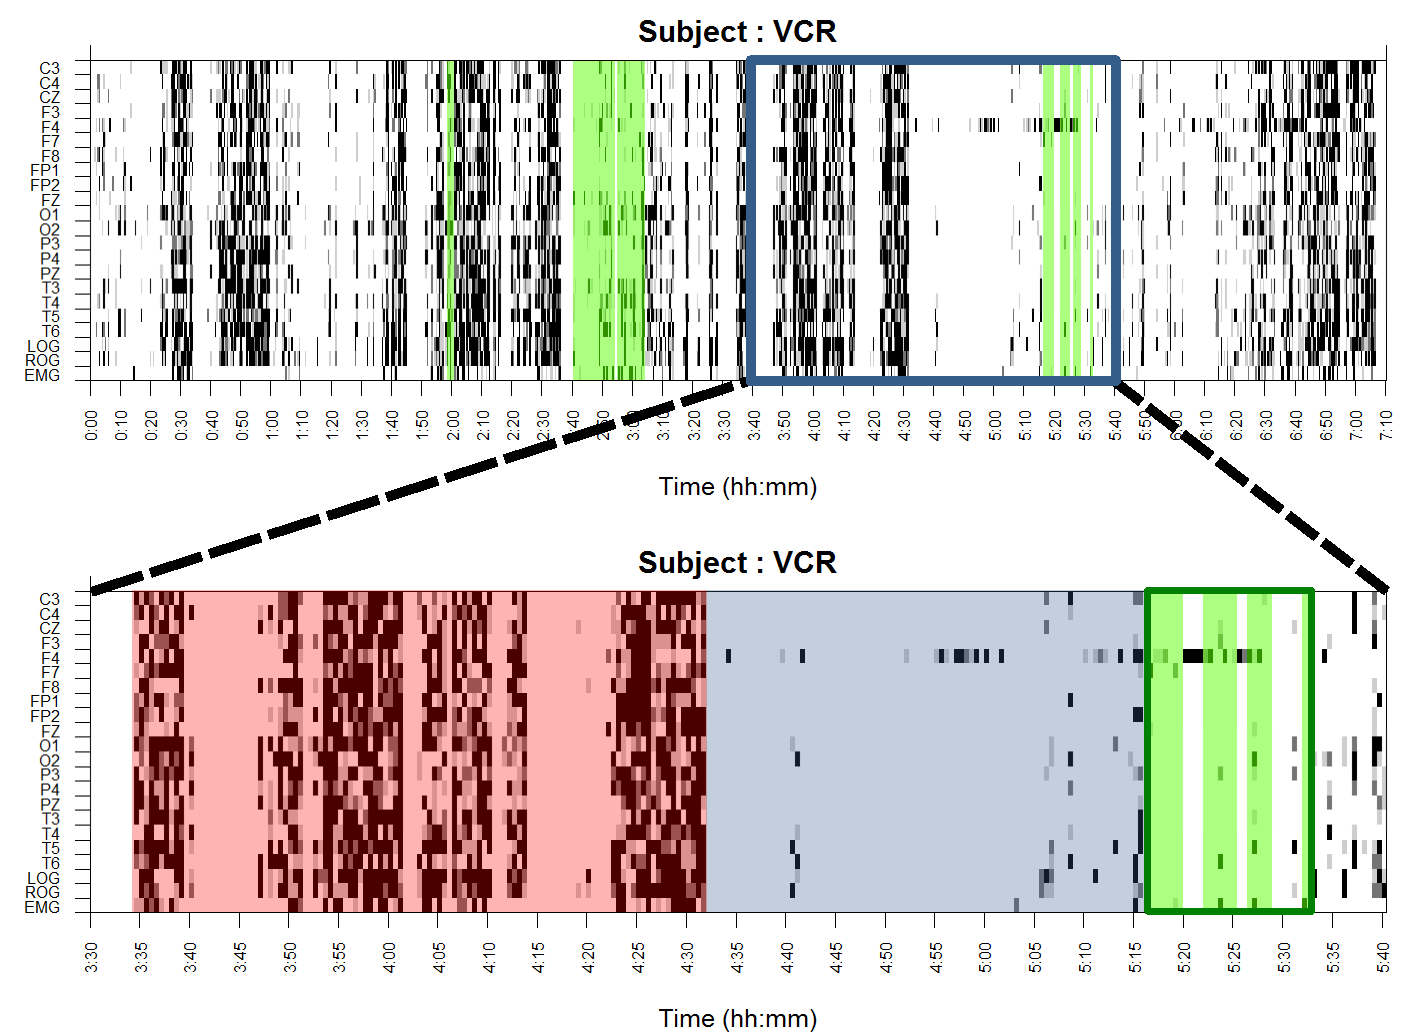
\includegraphics[width=0.95\textwidth]
{./img_ejemplos/zoom_VCR.pdf}
\caption{Test}
\label{test1}
\end{figure}

\begin{figure}
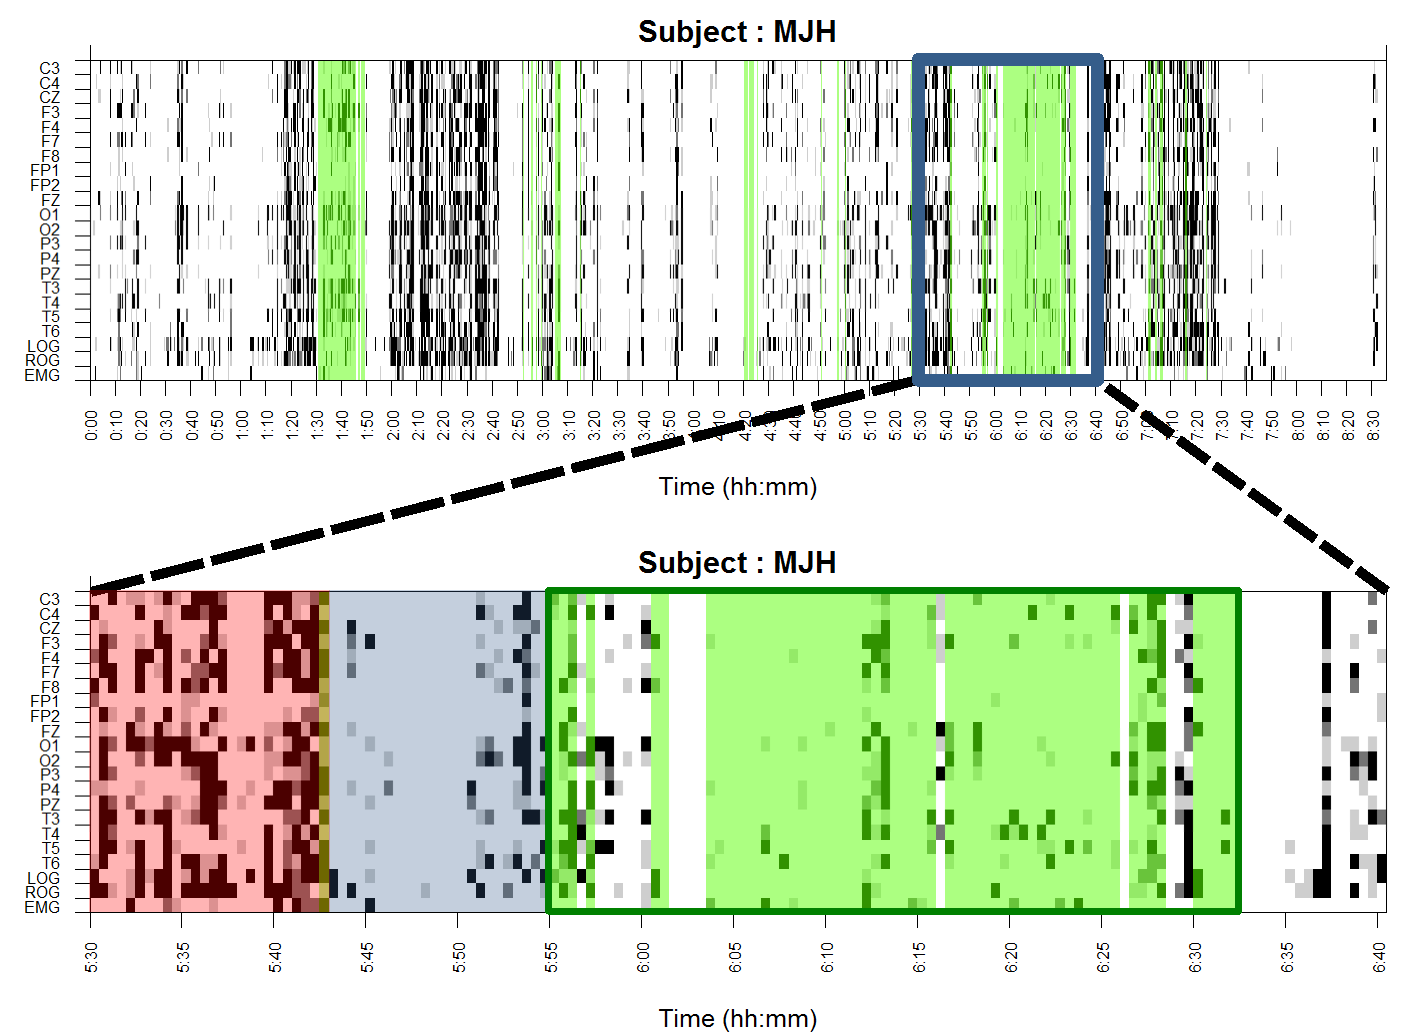
\includegraphics[width=0.95\textwidth]
{./img_ejemplos/zoom_MJH.pdf}
\caption{Test}
\label{test2}
\end{figure}

\begin{figure}
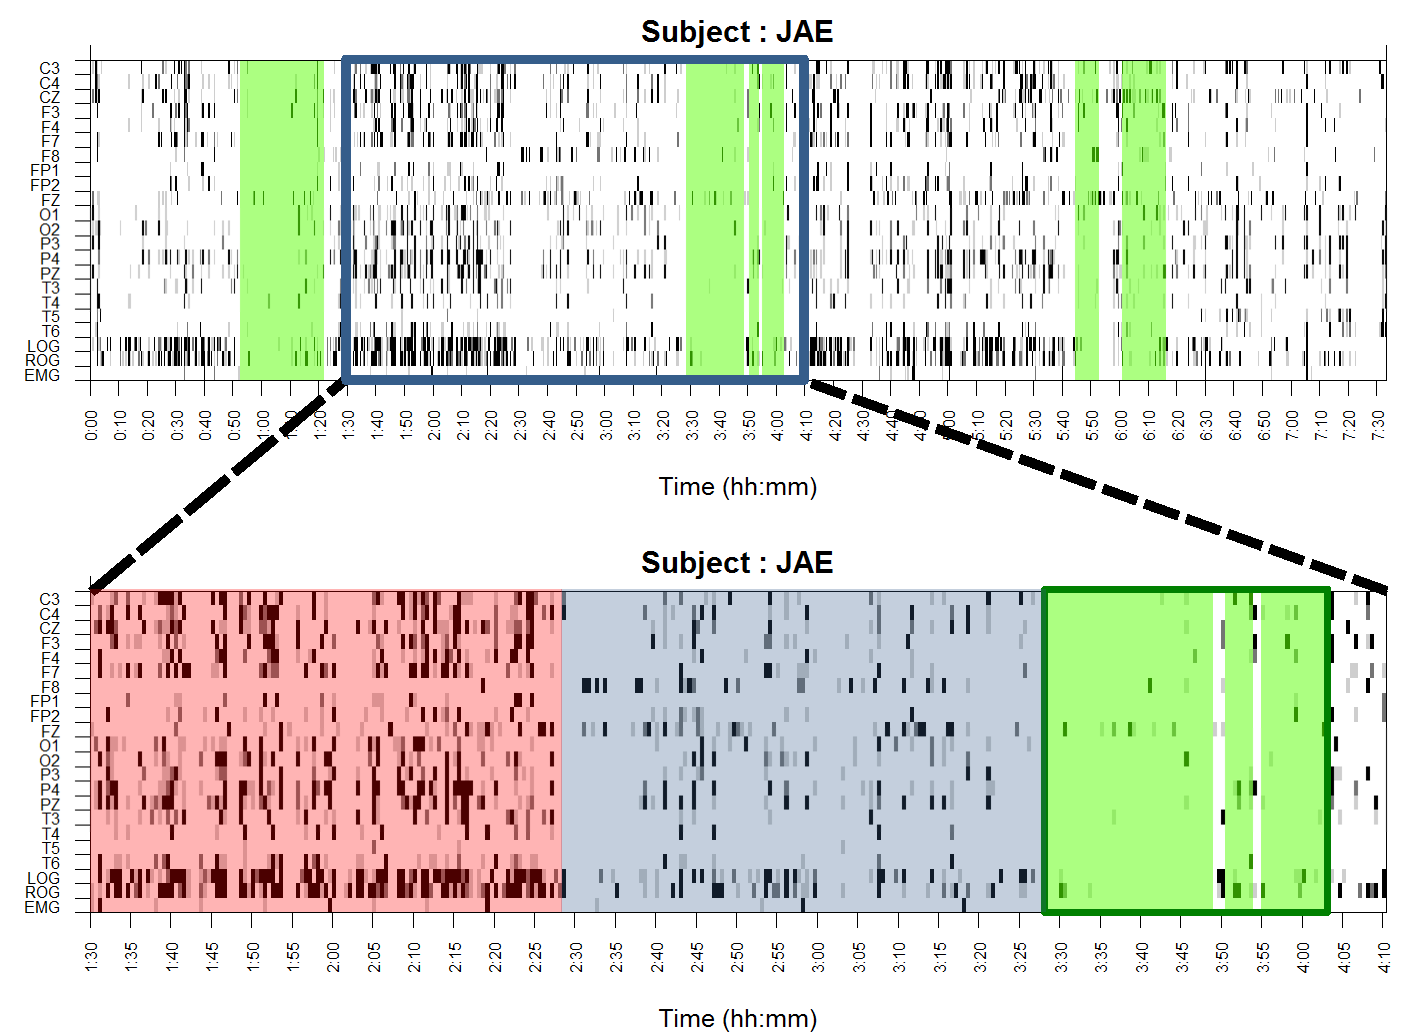
\includegraphics[width=0.95\textwidth]
{./img_ejemplos/zoom_JAE.pdf}
\caption{Test}
\label{test3}
\end{figure}

\begin{figure}
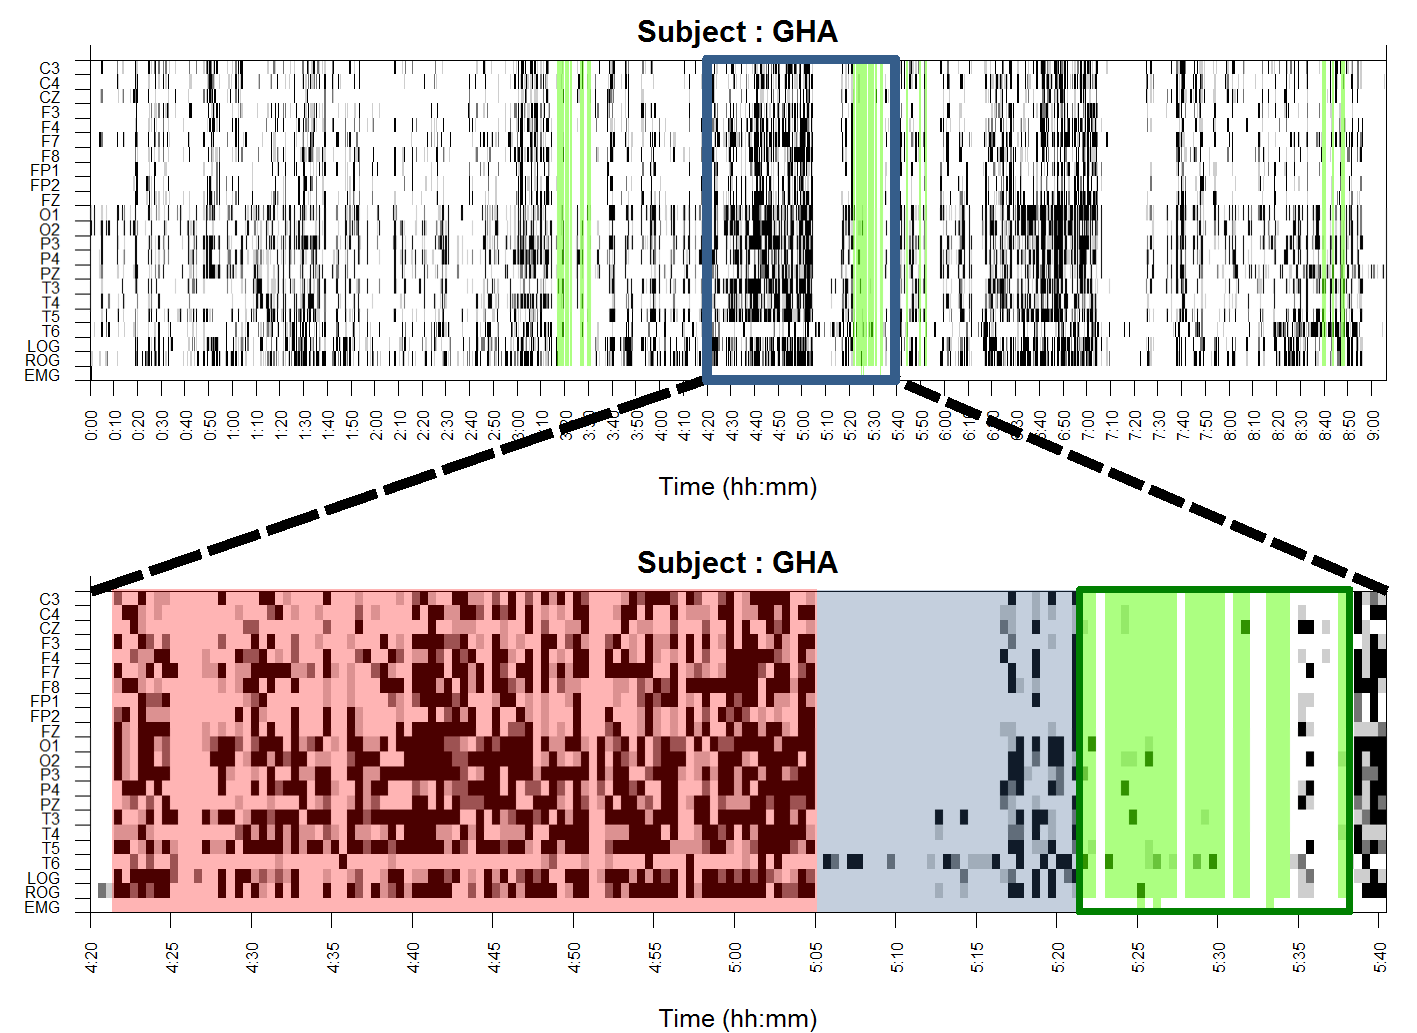
\includegraphics[width=0.95\textwidth]
{./img_ejemplos/zoom_GHA.pdf}
\caption{Test}
\label{test4}
\end{figure}


\begin{figure}
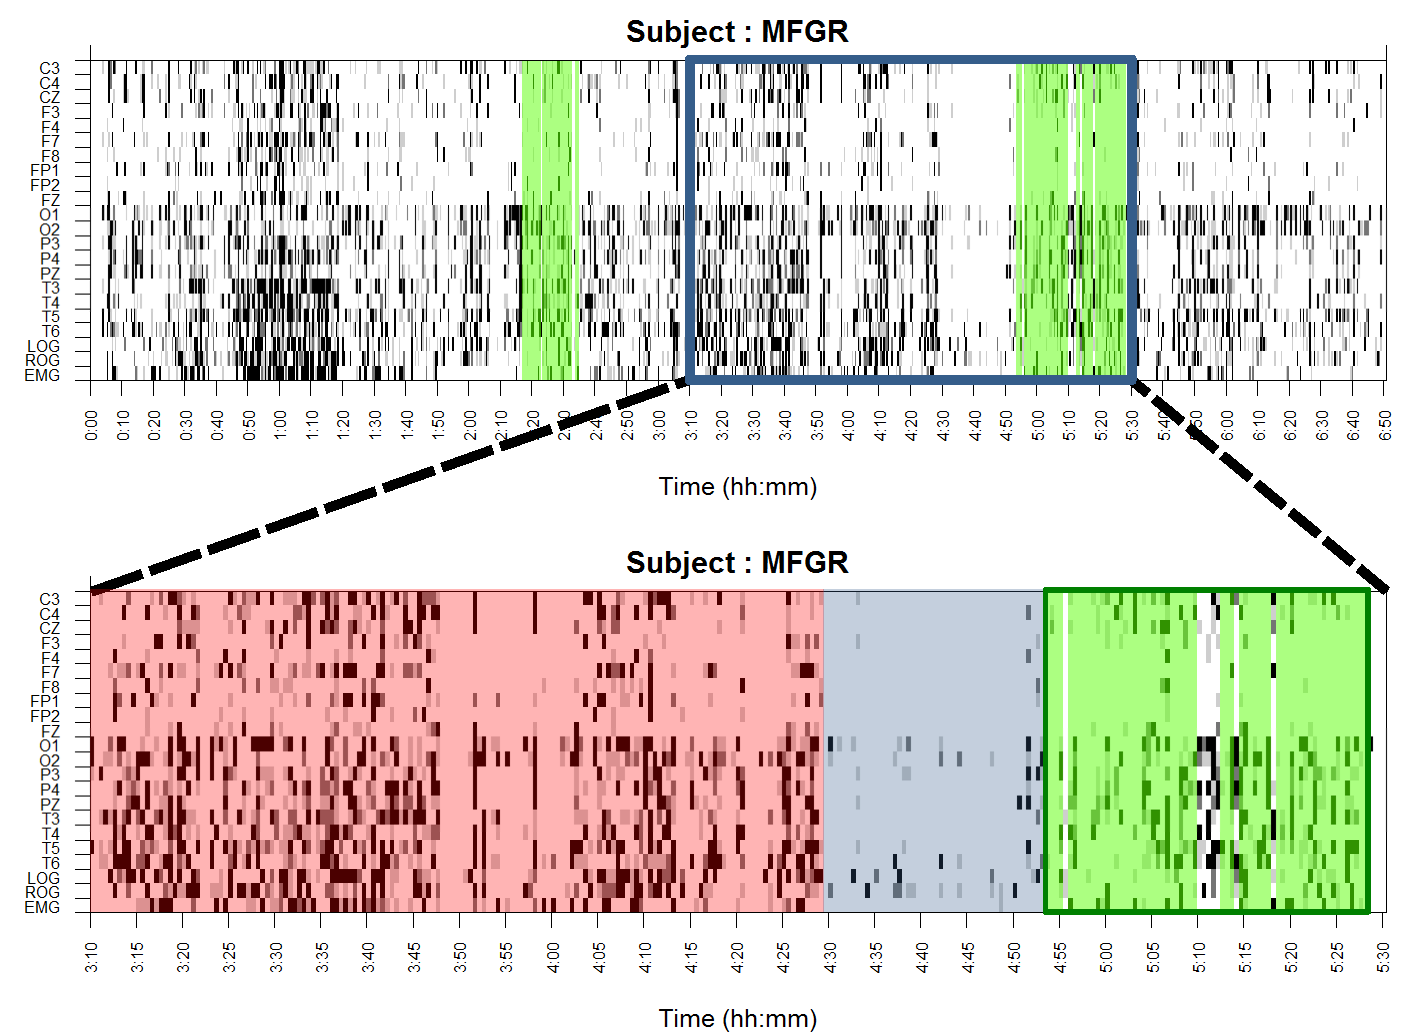
\includegraphics[width=0.95\textwidth]
{./img_ejemplos/zoom_MFGR.pdf}
\caption{Test}
\label{test5}
\end{figure}

%%%%%%%%%%%%%%%%%%%%%%%%%%%%%%%%%%%%%%%%%%%%%%%%%%%%%%%%%%%%%%%%%%%%%%%%%%%%%%%%%%%%%%%%%%%%%%%%%%%%
%%%%%%%%%%%%%%%%%%%%%%%%%%%%%%%%%%%%%%%%%%%%%%%%%%%%%%%%%%%%%%%%%%%%%%%%%%%%%%%%%%%%%%%%%%%%%%%%%%%%
%%%%%%%%%%%%%%%%%%%%%%%%%%%%%%%%%%%%%%%%%%%%%%%%%%%%%%%%%%%%%%%%%%%%%%%%%%%%%%%%%%%%%%%%%%%%%%%%%%%%
%%%%%%%%%%%%%%%%%%%%%%%%%%%%%%%%%%%%%%%%%%%%%%%%%%%%%%%%%%%%%%%%%%%%%%%%%%%%%%%%%%%%%%%%%%%%%%%%%%%%
